\newpage
\section{Results}
This section will give some simple examples of the previously described system to illustrate the implications of the barrier fluctuations coupled to the diffusive transport of Brownian particles.\\
It will also give a close examination of certain limits e.g. of very fast and very slow barrier fluctuations and compare these to simulation results. In addition, it will be evaluated if the solution for a step shaped barrier is a valid approximation for smooth potentials of similar shape depending on the timescale of the barrier fluctuations. \\
Finally it will show the effects that come from the transition of the barrier between two states due to independent variation of its HIGH $\rightarrow$ LOW and LOW $\rightarrow$ HIGH switching rates.
\section{A Two State Barrier with Symmetric Switching Rates}
The first example will be the most simple system possible consisting only of a two state barrier of hight $U_1 = 0$ and $U_2 \ne 0$ that is ether on or off. Also the barrier switching is symmetric i.e. the on $\rightarrow$ off and off $\rightarrow$ on rates are equal $\mathbb{W}_{12}=\mathbb{W}_{21}=W$ such that the potential of mean force acting on the Brownian particles is independent of the switching rate.
This allows for the detailed study of effects solely coming from the coupling of timescales between barrier fluctuations and diffusive transport without any other influence.
\subsection{Particle Density}
The first step for the investigation of the example is the calculation of the analytic solution for the density profiles of the Brownian particles. Therefore one first writes down the corresponding Fokker-Planck equation:
\begin{align}
    \frac{\partial \rho_1(r,t)}{\partial t} &= \vec \nabla \left[ D \vec \nabla \rho_1(r,t) \right] - W_{2,1}\rho_1(r,t) + W_{1,2}\rho_2(r,t) \nonumber \\
    \frac{\partial \rho_2(r,t)}{\partial t} &= \vec \nabla \left[\rho_2(r,t) \vec \nabla \frac{U_2(r)}{\gamma} + D \vec \nabla \rho_2(r,t) \right] - W_{1,2}\rho_2(r,t) + W_{2,1}\rho_1(r,t)
    \label{two_state_fpe}
\end{align}
Note that the particles in state $m=1$ move freely and are not subject to any potential barrier. 
Since the transition rates are symmetric $W_{1,2} = W_{2.1} = W$  the transition rate matrix has the form:
\begin{equation}
    \mathbb{W} = \left( \begin{array}{rr}
    W & -W \\
    -W & W 
\end{array} \right)
    \label{two_state_transition_matrix}
\end{equation}
With eigenvalues $\lambda_1 = 0$ and $\lambda_2 = -2W$. The steady state solution to the transition matrix is 
\begin{equation}
    \vect{\rho}^{(eq)}=\left(\frac{1}{2}, \frac{1}{2}\right)^{T}
    \label{rhoeq}
\end{equation}
which obviously satisfies the detailed balance property \eqref{detailed_balance}. \\
The diagonal form of equation \eqref{two_state_fpe} is now 
\begin{equation}
    \frac{\partial}{\partial t} \tilde{\vect{\rho}} = \left( \begin{array}{ll}
        D\vec{\nabla}^{2} & 0 \\
        0 & D\vec{\nabla}^{2} - 2W
    \end{array} \right) \tilde{\vect{\rho}}
    \label{fpmeq5}
\end{equation}
and the steady state solution in terms of eigenfunctions of $\mathbb{W}$ reads
\begin{align}
    \tilde{\rho}_1^{(k)} &= c_{1,1}^{(k)} + \frac{c_{1,2}^{(k)}}{r} \\
    \tilde{\rho}_2^{(k)} &= \frac{c_{2,1}^{(k)}}{r}{\rm exp}\left[-\frac{r}{r_d}\right]+ \frac{c_{2,2}^{(k)}}{r}{\rm exp}\left[\frac{r}{r_d}\right]
    \label{ind_sol_U2}
\end{align}
With the previously defined decay length $r_d$:
\begin{equation}
    r_d = \sqrt{\frac{d}{2W}}
    \label{rd_two_state}
\end{equation}
Once the coefficients $c^{(k)}_{i,j}$ are calculated from the boundary and fit conditions the density profiles can be plotted for several sets of parameters. If not stated differently, the parameters are given by the values in the following table. The choice of parameters is arbitrary now since the influence of each of them will be examined separately in later parts of this section.
\begin{equation}
    \begin{array}{r|l}
        Parameter & Value \\ \hline
        R_s & 1 \\
        a   & 6 \\
        b   & 11 \\
        U_2/K_B T & \mp 3 \\
    \end{array} \nonumber
    \label{Parameters}
\end{equation}
The first parameter that will be studied is the decay length $r_d$. The easiest way to get a first impression of its influence is to look at the density profiles. Therefore several examples for different parameter choices are given next.
For illustrative reasons the total particle density is normalized to $\rho_{tot}^{(eq)}=2$ for $r \rightarrow \infty$ in the following plots and the particle densities in the different states are depicted together with the mean particle density. \\
Since the state of the barrier can also be treated as a property of the Brownian particles as discussed in section \ref{Model_Description} it is convenient do so for the following discussion. The particles that are influenced by the barrier will hence be called \emph{active} whereas the particles that are not will be called \emph{inactive}. \\ In the following density plots the density of active particles is depicted in blue while the density of the inactive particles is depicted in red.

\begin{minipage}[t]{0.5 \textwidth}
    \begin{figure}[H]
        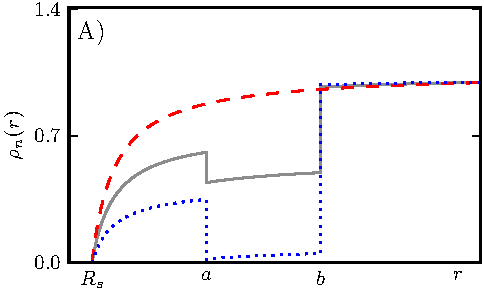
\includegraphics[width = 1 \textwidth]{plots/d1.pdf}
    \end{figure}
\end{minipage}
\begin{minipage}[t]{0.5 \textwidth}
    \begin{figure}[H]
        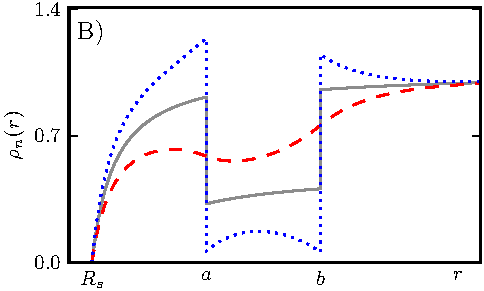
\includegraphics[width = 1 \textwidth]{plots/d2.pdf}
    \end{figure}
\end{minipage}
\begin{minipage}[t]{0.5 \textwidth}
    \begin{figure}[H]
        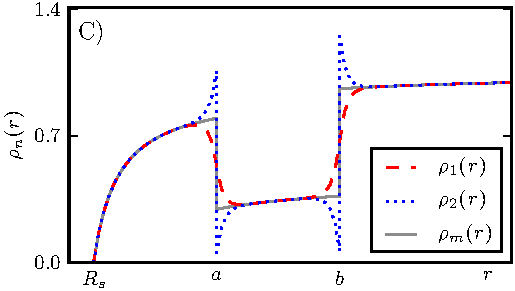
\includegraphics[width = 1 \textwidth]{plots/d3.pdf}
    \end{figure}
\end{minipage}\hspace{0.02\textwidth}\begin{minipage}[t]{0.48 \textwidth}
    \begin{figure}[H]
        \caption{Density profiles for repulsive fluctuating barrier. The densities of particles in state $m=1$ and state $m=2$ are depicted in dashed red, and dotted blue respectively. The decay length is given by A): $r_d = 25$, B): $r_d=2.5$ and C): $r_d=0.25$. \label{rep_symm_dens_profile}}
    \end{figure}
\end{minipage}


\begin{minipage}[t]{0.5 \textwidth}
    \begin{figure}[H]
        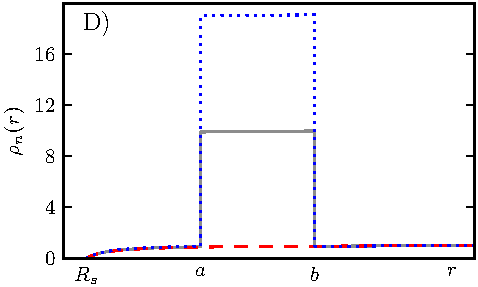
\includegraphics[width = 1 \textwidth]{plots/d4.pdf}
    \end{figure}
\end{minipage}
\begin{minipage}[t]{0.5 \textwidth}
    \begin{figure}[H]
        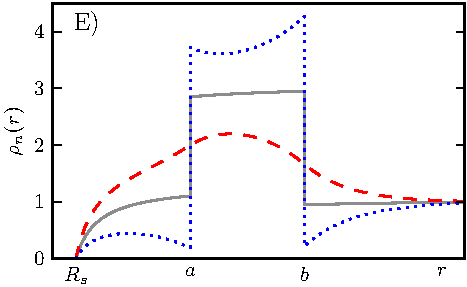
\includegraphics[width = 1 \textwidth]{plots/d5.pdf}
    \end{figure}
\end{minipage}
\begin{minipage}[t]{0.5 \textwidth}
    \begin{figure}[H]
        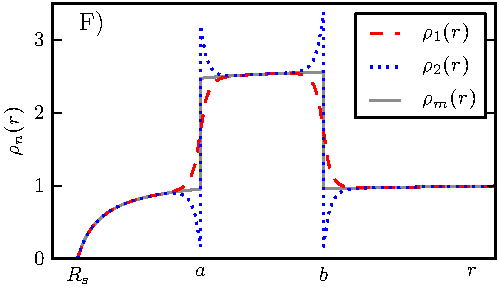
\includegraphics[width = 1 \textwidth]{plots/d6.pdf}
    \end{figure}
\end{minipage}\hspace{0.02\textwidth}\begin{minipage}[t]{0.48 \textwidth}
    \begin{figure}[H]
        \caption{Density profiles for attractive fluctuating barrier. The densities of particles in state $m=1$ and state $m=2$ are depicted in dashed red, and dotted blue respectively. The decay length is again given by A): $r_d = 25$, B): $r_d=2.5$ and C): $r_d=0.25$\label{att_symm_dens_profile}}
    \end{figure}
\end{minipage} 
\newpage
This case neatly illustrates the role of $r_d$ as the persistence length of the influence of the potential fluctuations. For distances $d_a = |r - a|$ and $d_b = |r - b|$ far from the jump discontinuities of the potential $d_a, d_b >> r_d$ the thermal motion of the Brownian particles dampens the influence of the potential barrier and the densities of active and inactive particles converge to the same value again.\\
So if $r_d$ is much larger as the overall spacing of the potential barrier the particles in different states are mostly independent from each other. If $r_d$ is much smaller than the spacing of the barrier the particle densities are equal except for a small around the barrier borders that is approximately $r_d$ wide.\\
The interesting behaviour emerges if the decay length is approximately of the same order as the barrier spacing. Then the densities of the different particles species are not independent of each other over the entire width of the system. This somehow has the effect that the average particle density at the inside of the barrier unexpectedly high. \\
This is curious and worth a closer look. Therefore, in the following the underlying mechanism and its implications on the reaction rate will be thoroughly examined. \\ 

\newpage
\subsection{Flow Analysis}
Density profiles only give information about where particles are. However, it is of interest how they got there and where they are going next. Therefore it is reasonable to use particle fluxes for a further study of the system. \\
To do so the radial coordinate of the system is divided into different areas as depicted in figure \ref{fig:flowchart_scetch}.
\begin{figure}[H]
    \centering
    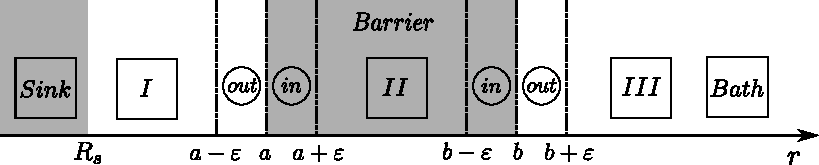
\includegraphics[width = .9 \textwidth]{plots/drawing.pdf}
    \caption{sketch of the spatial discretization for the flow analysis of the system: The Sink and the Barrier are marked in gray. The circles represent narrow volumes of width $\varepsilon$ right at the barrier borders. $\varepsilon$ is set to be one tenth of the barrier width. The squares represent the large spaces between barrier and sink ($I$), between the sink boundaries ($II$) and outside the sink ($III)$. Each volume has the shape of a spherical shell (except the sink which is a sphere). Active and inactive particles are investigated separately in each of these volumes}
    \label{fig:flowchart_scetch}
\end{figure}
For each of these areas one examines the spatial fluxes from and to neighbouring areas and the reactive fluxes from one particle state to the other. \\
For this purpose it is convenient to use the integral form of the continuity equation derived in \eqref{ce0}. To employ it in the actual problem one takes the density profiles to be constant in time such that its left hand side vanishes. Then the terms on the right hand side are calculated separately. The spatial fluxes at the volume boundaries:
\begin{equation}
    J_m^{(S)}(r_i) = \int_{r_i} \vec{j}_m(r) {\rm d} \vec{A}
    \label{spatial_flux}
\end{equation}
and the reactive fluxes from one particle species to the other:
\begin{equation}
    J_{mm'}^{(R)}(r_i,r_j) =\int_{r_i}^{r_j} \left\{ \mathbb{W}_{m'm}\rho_m - \mathbb{W}_{mm'} \rho_{m'} \right\} {\rm d} r
    \label{reaction_flux}
\end{equation}
where $r_i$ and $r_j$. are the radii $R_s$, $a-\varepsilon$, $a$ etc. of the spatial discretization given in figure \ref{fig:flowchart_scetch}.
These fluxes are then represented as arrows between the icons representing the corresponding areas as illustrated in figure \ref{fig:flowchart_scetch}. Active and inactive particles are depicted separately where the icons representing active particles are blue and the icons representing inactive particles are red. \\ \textbf{Interpreting the following flow diagrams it is important to note, that the flows depicted by the arrows are normalized to the largest value for each example. Therefore the arrows only represent \emph{relative importance of fluxes} and have no meaning for their absolute values!} \newpage
. \\ \vspace{-2 cm}

\begin{minipage}[t]{.372 \textwidth}
    \vspace{0.5 cm}
    \begin{figure}[H]
        \caption{Flow diagram for repulsive barrier: This plot shows spatial and reactive particle flows between different particle species (active particles are represented in blue, inactive particles are represented in blue) and different spatial regions (see figure \ref{fig:flowchart_scetch} for reference) for the examples given in figure \ref{rep_symm_dens_profile}. The difference between the different plots is again the decay length which is equal to \newline A): $r_d=25$, B): $r_d=2.5$ and \newline C): $r_d = 0.25$.
    \label{fig:flow_repulsive}}
    \end{figure}
\end{minipage}\hspace{0.02 \textwidth}\begin{minipage}[t]{.608 \textwidth}
    \begin{figure}[H]
        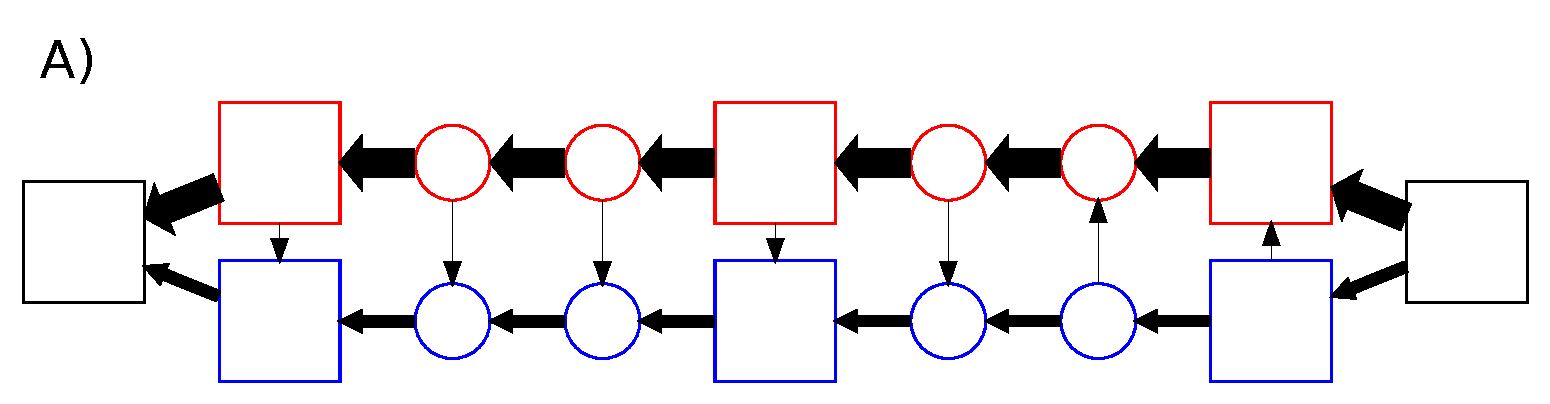
\includegraphics[width = 1 \textwidth]{plots/rep_flowchart0.pdf} 
        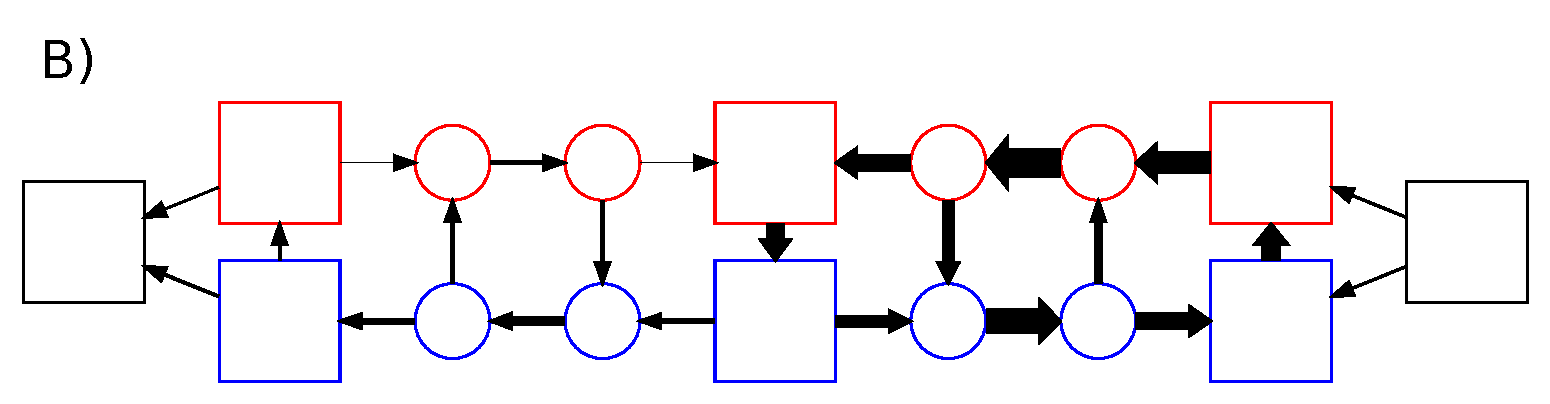
\includegraphics[width = 1 \textwidth]{plots/rep_flowchart1.pdf} 
        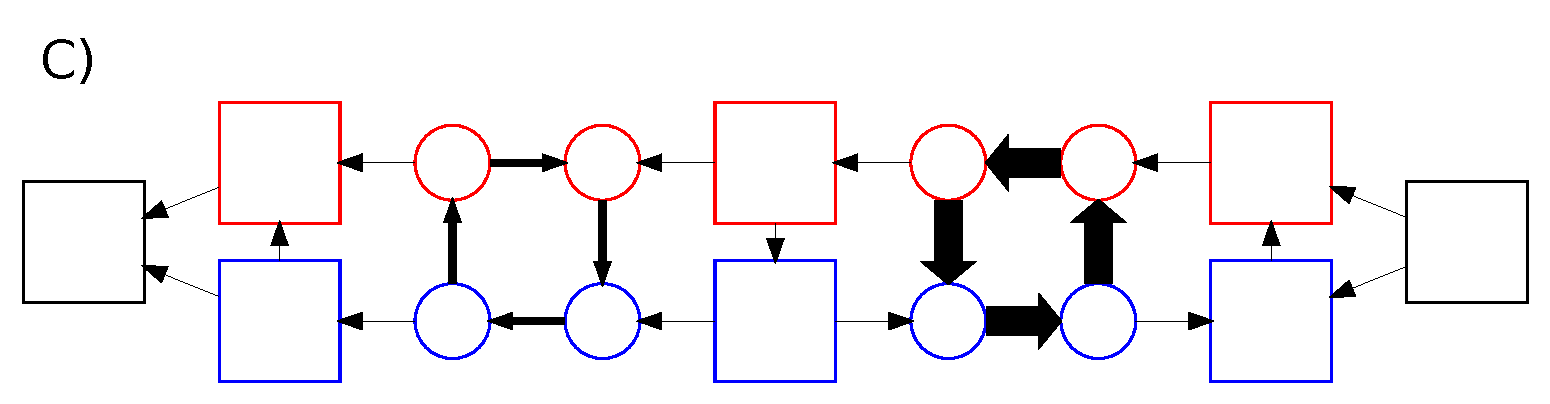
\includegraphics[width = 1 \textwidth]{plots/rep_flowchart2.pdf}
    \end{figure}
\end{minipage}
\vspace{0.5 cm} \\
It is obvious from this illustration that the system behaves qualitatively different depending on its the decay length.
\begin{itemize}
    \item For long decay length as in figure \ref{fig:flow_repulsive} A) it is visible from the very narrow arrows connecting red and blue icons that the particles in both states are independent in good approximation. Therefore inactive particles are not hindered by the barrier on their way from the bath to the sink whereas active particles have to overcome the potential barrier and are thus less likely to interact with the sink. Ether way, particles are very unlikely to change their state in the process. 
    \item For short decay length as in figure \ref{fig:flow_repulsive} C) The behavior is clearly different. Particle movement is closely tied to the potential boundaries at $r=a$ and $r=b$. There active particles are very likely to cross the boundary in downward direction only. Therefore the potential drives a spatial selection of particles that leads to an excess of active particles right outside and a deficit of active particles inside the barrier. The resulting difference in concentration of active and inactive particles at both sides of the barrier boundary leads to a strong reactive fluxes. Inside the barrier particles switch from inactive (red) to active (blue) and outside the barrier they switch from active to inactive state. The resulting imbalance of inactive particles draws them across the barrier from the out to the inside. As obvious from the flow diagram, the result is a strong \emph{circular current}. Since most of the particles switch states before they can diffuse more than $r_d$ away, the process is closely tied to the barrier boundaries. 
    \item For medium decay length as in figure \ref{fig:flow_repulsive} B) These circular currents are still existent but not so closely tied to the boundaries of the barrier. Therefore they they overlap in space. This has the effect that once a particles has crossed the outer boundary of the barrier as part of one circular current it can switch to the other circular current to cross the inner boundary of the barrier. 
\end{itemize}
In the case of an attractive potential barrier the processes at work are quite similar. The differences to the repulsive case are outlined on the basis of the following flow diagrams: \vspace{-.5 cm} \\
\begin{minipage}[t]{.372 \textwidth}
    \vspace{.5 cm}
    \begin{figure}[H]
        \caption{Flow diagram for attractive barrier: This plot shows spatial and reactive particle flows between different particle species (active particles are represented in blue, inactive particles are represented in blue) and different spatial regions (see figure \ref{fig:flowchart_scetch} for reference) for the examples given in figure \ref{att_symm_dens_profile}. The difference between the different plots is again the decay length which is equal to \newline A): $r_d=25$, B): $r_d=2.5$ and \newline C): $r_d = 0.25$.
    \label{fig:flow_attractive}}
    \end{figure}
\end{minipage}\hspace{0.02 \textwidth}\begin{minipage}[t]{.608 \textwidth}
    \begin{figure}[H]
        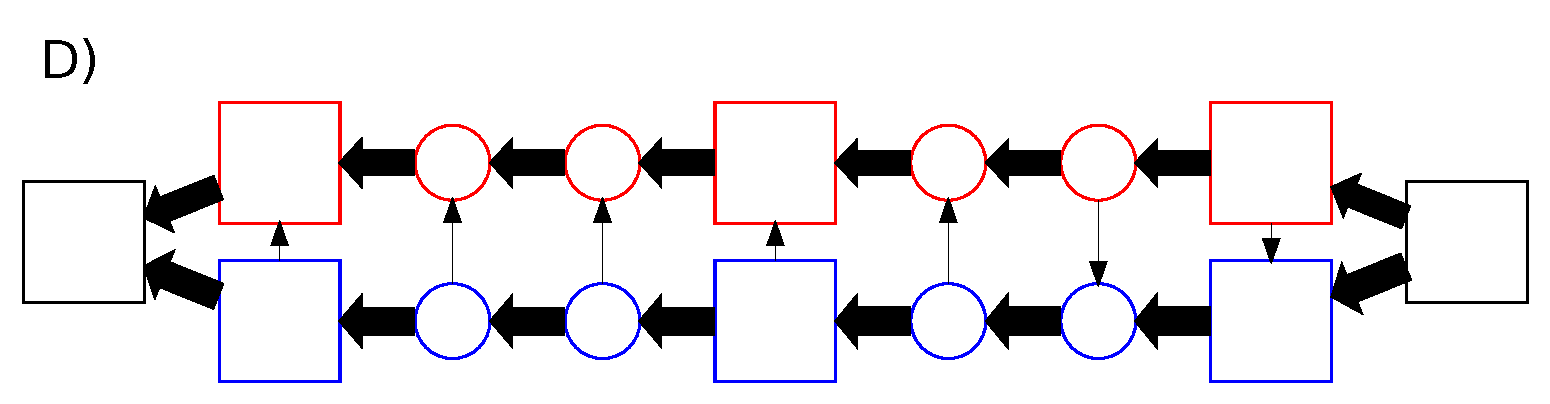
\includegraphics[width = 1 \textwidth]{plots/att_flowchart0.pdf}
        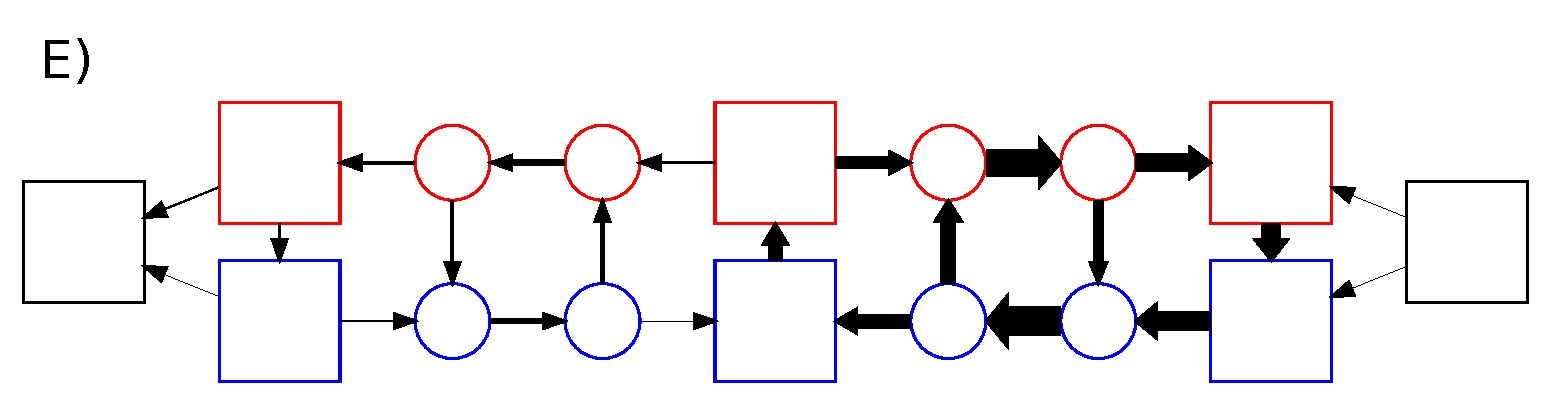
\includegraphics[width = 1 \textwidth]{plots/att_flowchart1.pdf}
        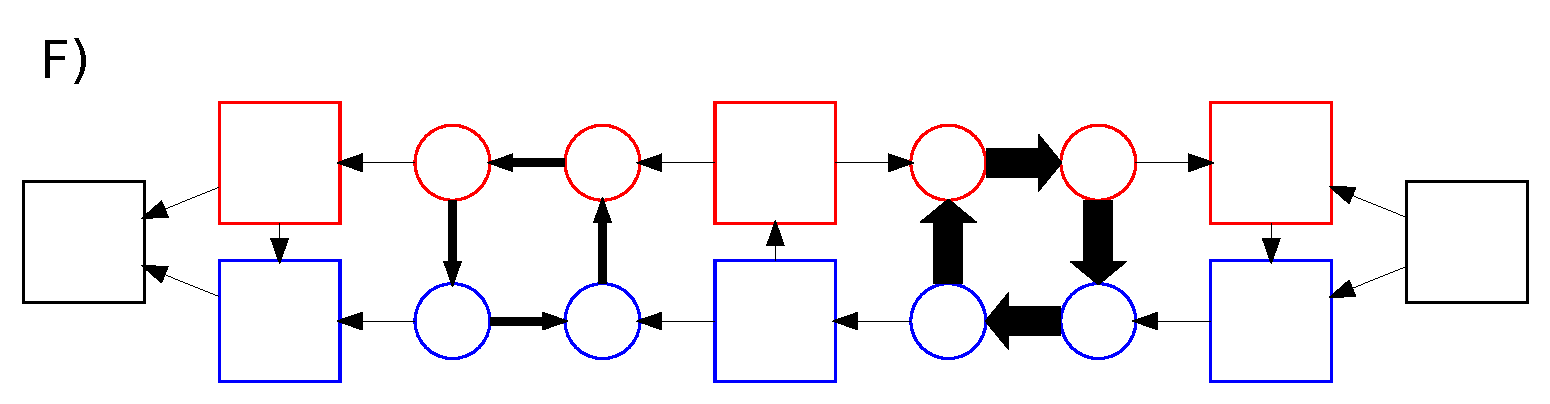
\includegraphics[width = 1 \textwidth]{plots/att_flowchart2.pdf}
    \end{figure}
\end{minipage}
\vspace{.5 cm} \\
The differences to the differences of these examples to the ones presented before in figure \ref{fig:flow_repulsive} can be pointed out one by one:
\begin{itemize}
    \item For long decay length as in figure \ref{fig:flow_attractive} D) the two particle species are independent from each other in good approximation. The difference to the former example is that the active particles are not hindered by the attractive barrier once the steady state is reached. They accumulate in the attractive potential until their concentration is high enough to to make it equally possible for particles to enter and leave the barrier (which es the essentially given by the probability for particles to enter the potential). Therefore both particle species do equally contribute to the flux of particles from the bath to the sink.
    \item For short decay length as in figure \ref{fig:flow_attractive} F) the system again shows strong circular currents around the boundaries of the potential barrier. The difference is here that if active particles now cross the barrier in downward direction this means from the ``out'' to the ``in'' side. Therefore the circular currents are now directed in the other direction (clockwise vs. counter clockwise in this representation)
    \item For medium decay length as in figure \ref{fig:flow_attractive} E)  the two circular currents overlap just as they do in the case of a repulsive barrier. Therefore it is again likely for active particles to be drawn across the outer border of the potential by one current and then cross the boundary of the inner barrier as part of the other current.
\end{itemize}
This analysis has shown how the system behaves qualitatively different depending on switching rate of the barrier or rather depending on the decay length of the particle densities. Knowing this, it is now time to turn to the key quantity in this investigation which is the reaction rate of particles interacting with the sink. 
\subsection{Reaction Rates}

The calculation of the reaction rate as outlined in section \ref{Reaction_Rates_over_Fluctuating_Barriers} leads to the following expression. The index of $\alpha_2$ will be omitted for reasons of convenience.
\begin{align}
    \frac{K}{K_{Debye}} &= \frac{F_1}{F_2}
    \label{two_state_rate}
\end{align}
$F_1$ and $F_2$ denote the following expressions:
\begin{align*}
    F_1 =& 2 \left(a \left(\alpha-5 b \alpha^2\right)+b \alpha-1\right) e^{2 \alpha (a+b)+u}-2 (a \alpha+1) (b \alpha-1) e^{2 (b+1) \alpha+u}-4 b \alpha (b \alpha+1) e^{3 a \alpha+b \alpha+u} \\
    &+2 b \alpha (b \alpha+1) e^{3 a \alpha+b \alpha+2 u}+4 b \alpha (b \alpha+1) e^{\alpha (a+b+2)+u}-2 b \alpha (b \alpha+1) e^{\alpha (a+b+2)+2 u} \\
    &-2 (a \alpha-1) (b \alpha+1) e^{4 a \alpha+u}+(a \alpha-1) (b \alpha+1) e^{4 a \alpha+2 u}-2 (a \alpha+1) (b \alpha+1) e^{2 (a+1) \alpha+u} \\
    &-(a \alpha+1) (b \alpha+1) e^{2 (b \alpha+u+\alpha)}-(3 a \alpha-1) (b \alpha+1) e^{2 (\alpha (a+b)+u)} \\
    &+(3 a \alpha+1) (b \alpha+1) e^{2 (a \alpha+u+\alpha)}-2 b \alpha (b \alpha+1) e^{\alpha (a+b+2)}+2 b \alpha (b \alpha+1) e^{\alpha (3 a+b)} \\
    &+e^{4 a \alpha} (a \alpha-1) (b \alpha+1)-e^{2 (a+1) \alpha} (a \alpha-1) (b \alpha+1)+(a \alpha+1) e^{2 (b+1) \alpha} (3 b \alpha-1) \\
    &-(a \alpha+1) (3 b \alpha-1) e^{2 \alpha (a+b)} \\
    F_2 =& -4 \alpha \left(a^2 \alpha-a \alpha+a-b \alpha-2\right) e^{\alpha (a+b+2)+u}+2 \alpha \left(a^2 \alpha-a \alpha+a-b \alpha-2\right) e^{\alpha (a+b+2)+2 u} \\
    &-4 \alpha \left(a^2 \alpha-a (\alpha+1)+b \alpha+2\right) e^{3 a \alpha+b \alpha+u}+2 \alpha \left(a^2 \alpha-a (\alpha+1)+b \alpha+2\right) e^{3 a \alpha+b \alpha+2 u} \\
    &+2 \alpha e^{\alpha (a+b+2)} \left(a^2 \alpha-a \alpha+a-b \alpha-2\right)+2 \alpha e^{\alpha (3 a+b)} \left(a^2 \alpha-a (\alpha+1)+b \alpha+2\right) \\
    &-\left(3 \alpha^2 (a (b-2)+2 b)+\alpha (a-3 b+4)-1\right) e^{2 (\alpha (a+b)+u)} \\
    &-2 \left(\alpha^2 (a (5 b+2)-2 b)+\alpha (a+b-4)+1\right) e^{2 \alpha (a+b)+u} \\
    &+2 (a \alpha+1) ((b-2) \alpha+1) e^{2 (b+1) \alpha+u}+2 ((a-2) \alpha-1) (b \alpha+1) e^{2 (a+1) \alpha+u} \\
    &-2 (a \alpha-1) (b \alpha+1) e^{4 a \alpha+u}+(a \alpha-1) (b \alpha+1) e^{4 a \alpha+2 u}+((a+2) \alpha+1) (b \alpha+1) e^{2 (a \alpha+u+\alpha)} \\
    &-(a \alpha+1) ((3 b-2) \alpha+1) e^{2 (b \alpha+u+\alpha)}-e^{2 \alpha (a+b)} \left(\alpha^2 (a (3 b+2)-2 b)+\alpha (-3 a+b+4)-1\right) \\
    &+e^{4 a \alpha} (a \alpha-1) (b \alpha+1)-e^{2 (a+1) \alpha} ((3 a-2) \alpha-1) (b \alpha+1)+(a \alpha+1) e^{2 (b+1) \alpha} ((b+2) \alpha-1)
\end{align*}
Sadly, this form of the solution does not tell us very much about the behaviour of the system. For a first impression, we will give some plots of the reaction rate vs. the persistence length of the solution using the parameters given above if not stated differently.\\
\begin{minipage}[t]{0.7 \textwidth}
    \begin{figure}[H]
        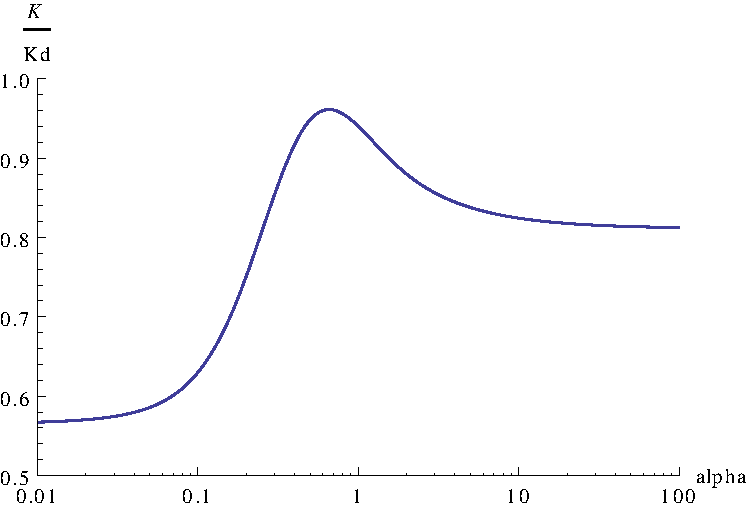
\includegraphics[width = 1 \textwidth]{plots/rate1.pdf}
    \caption{Reaction rate vs. switching rate for repulsive barrier}
    \label{fig:finite_barrier_rate+}
    \end{figure}
\end{minipage}\begin{minipage}[t]{0.3 \textwidth}
The plot on the left shows the reaction rate relative to the reaction rate of the ungated Debye problem for a fluctuating potential barrier of hight $[U_1 = 0, U_2 = 4]$. It is obvious that it shows some sort of resonant behaviour. The reaction rate converges to some constant, finite values lower than the ungated rate and is maximised by a certain ratio of switching rate and diffusion constant. For certain parameters the rate at its maximum is even higher higher than the rate of the ungated problem.
\end{minipage}
\par
\begin{minipage}[t]{0.7 \textwidth}
    \begin{figure}[H]
        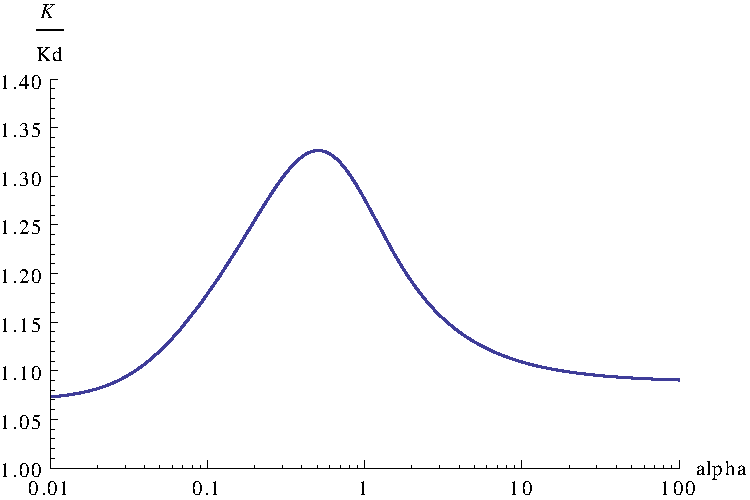
\includegraphics[width = 1 \textwidth]{plots/rate2.pdf}
    \caption{Reaction rate vs. switching rate for attractive barrier}
    \label{fig:finite_barrier_rate-}
    \end{figure}
\end{minipage}\begin{minipage}[t]{0.3 \textwidth}
This plot shows the quotient of the reaction rates of the gated and the ungated Debye problem for an attractive fluctuating potential barrier of hight $[U_1 = 0, U_2 = -4]$. Under these conditions the reaction rate of the gated problem is always higher than the one of the ungated problem. Similar to the behaviour emerging from a repulsive barrier the rate is maximised at a certain ratio of switching rate and diffusion constant. The reaction rate at the maximum is
thereby\end{minipage}
considerably higher than at the limiting cases for very fast and very slow switching of the barrier. Comparing the repulsive barrier and the attractive barrier setting it is apparent, that the limiting cases for $\gamma/D \rightarrow 0$ and $\gamma/D \rightarrow \infty$ do differ considerably in the first case whilst in the second they do not. \par
Next we investigate if this kind of resonant activation does always occur or only for certain parameters. Therefore we calculate approximate expressions for the limiting behaviour of the reaction rate.

\subsection{Slow Fluctuation Limit}
For slow fluctuations of the potential barrier the decay length $r_d$ and therefore the spatial influence of the potential barrier becomes large compared to the length scale of the system. This is equivalent with the fact, that the diffusion time of the substrate particles across the system is much smaller than the inverse switching rate of the potential barrier. 
To evaluate this limit, we use eq. \eqref{two_state_fpe} with symmetric rates take the limit of $W \rightarrow 0$ and consider the steady state case.
This results in two independent equations for the two states of the potential:
\begin{align}
    \frac{\partial \rho_1(r,t)}{\partial t} &= \vec \nabla \left[ D \vec \nabla \rho_1(r,t) \right] \\ \nonumber
    \frac{\partial \rho_2(r,t)}{\partial t} &= \vec \nabla \left[\rho_2(r,t) \vec \nabla \frac{U_2(r)}{\gamma} + D \vec \nabla \rho_2(r,t) \right]
    \label{two_state_fpe_W_to_0}
\end{align}
Where $U_2$ has the form given in \eqref{step_potential}.
The reaction rates for these independent equations can be calculated using the expressions given in \eqref{steady state ideal rate} and \eqref{K_Debye}. If one takes the detailed balance assumption for $r \rightarrow \infty$ to be still valid the combined rate can be calculated as the weighted average of the two independent rates. Since we the transition rates are taken to be symmetric, this results in:
\begin{align}
    K &= \frac{1}{2} \left[ 4 \pi D R_s^2 + 4 \pi D  \left\{\int_{R_s}^{\infty} \frac{\exp \left[ \frac{U_2(r')}{K_B T}\right]}{r'^2} \rm d r' \right\}^{-1} \right] \\ \nonumber
    &= 2 \pi D \left[ R_s^2 +\left\{\int_{R_s}^{a} \frac{1}{r'^2} \rm d r' + \int_{a}^{b} \frac{\exp \left[ \frac{U_2(r')}{K_B T}\right]}{r'^2} \rm d r' + \int_{b}^{\infty} \frac{1}{r'^2} \rm d r' \right\}^{-1} \right]
\end{align}
Now we evaluate the Integrals and divide by the Smoluchowski rate. Also $R_s$ and $K_B T $ are set to one such that the result is:
\begin{align}
    \frac{K}{K_{S}} &= \frac{1}{2} \left[1 + \left\{ 1 -\frac{1}{a} + \exp[U_2] \left(\frac{1}{a} - \frac{1}{b}  \right) + \frac{1}{b} \right\}^{-1} \right] \nonumber \\
    &= \frac{1}{2}\left[ 1 + \left\{ 1 + \left( \frac{1}{a} - \frac{1}{b} \right)\left( \exp[U_2] -1 \right) \right\}^{-1} \right] \nonumber \\
    &= \frac{1}{2} \left[ 1 + \left\{ 1 - \frac{(b - a)}{ab}\left(1 - \exp[U_2] \right) \right\}^{-1} \right] \nonumber \\
    &= \frac{1}{2} \left[ 1 + \frac{ab}{ab - \left( b-a \right)\left(1 - \exp[U_2] \right)} \right].
    \label{two_state_K_slow}
\end{align}
The result of this somewhat intuitive calculation can now be compared to the slow switching limit of eq. \eqref{two_state_rate}.
It proves to be sufficient to do a Taylor expansion around $\alpha_0 = 0$ to obtain
\begin{equation}
    \frac{K}{K_{S}} \approx \frac{(b-a)(1-e^u)-2ab }{2 \left((b-a) \left(1-e^u\right)-ab\right)} + \frac{  (b-a)^2\left(1-e^u\right)^2}{4 \left(ab + (b-a)(1-e^u)\right)^2} \alpha.
    \label{ksa}
\end{equation}
Where the leading therm can be modified to take the form
\begin{equation}
    \lim_{\alpha \rightarrow 0} \frac{K}{K_{S}} =\frac{1}{2}\left(1+ \frac{ab}{ab-(b-a) \left(1-e^u\right)}\right).
    \label{klim0a}
\end{equation}
This is exactly the result, that we obtained by the previous calculation.
\subsection{Fast Fluctuation Limit}
For fast fluctuations of the potential barrier, there is another way to deal with eq. \eqref{two_state_fpe}. In the limit of $W \rightarrow \infty$ the diffusion therm can be neglected compared to the reactive therms, such that in the case of symmetric rates $\rho_1(r) \equiv \rho_2(r) = \rho(r)$ holds for all $r>R_s$. Therefore both equations can be added resulting in 
\begin{equation}
    \frac{\partial \rho(r,t)}{\partial t} = \vec \nabla \left[\rho(r,t) \vec \nabla \frac{U_2(r)}{\gamma} + 2 D \vec \nabla \rho(r,t) \right]
    \label{fast_limit_fpe}
\end{equation}
Which is in fact equivalent to the case of a constant average potential barrier. In the steady state case this again reduces to
\begin{equation}
    0 = \vec \nabla \left[\rho(r,t) \vec \nabla \frac{U_2(r)}{2\gamma} + D \vec \nabla \rho(r,t) \right]
\end{equation}
such that the steady state rate can be calculated using the Debye formula:
\begin{align}
    K &=  4 \pi D \left\{\int_{R_s}^{\infty} \frac{\exp \left[ \frac{U_2(r')}{2 K_B T}\right]}{r'^2} \rm d r' \right\}^{-1} \nonumber \\
    &= 4 \pi D \left\{\int_{R_s}^{a} \frac{1}{r'^2} \rm d r' + \int_{a}^{b} \frac{\exp \left[ \frac{U_2(r')}{2K_B T}\right]}{r'^2} \rm d r' + \int_{b}^{\infty} \frac{1}{r'^2} \rm d r' \right\}^{-1}.
    \label{mean_potential_rate}
\end{align}
We evaluate the integrals, simplify and divide by the Smoluchowski rate to obtain
\begin{equation}
    \frac{K}{K_S} = \frac{ab}{ab - (b-a)(1-\exp\left[ \frac{U_2}{2} \right])}
    \label{K_fast_limit_false}
\end{equation}
where $R_s$ and $K_B T$ have been set to be one again. \\
Now a useful examination of the fast switching limit of eq. \eqref{two_state_rate} requires a bit more work.
To find the behaviour in the limit of $\alpha >>1$ we take a closer look at the different exponents that occur in the numerator and denominator of equation \eqref{two_state_rate}. Namely
\begin{align}
& e_1 = (3a+b)\alpha \nonumber \\
& e_2 = (2+2b)\alpha \nonumber \\
& e_3 = (2+a+b)\alpha \nonumber \\
& e_4 = 4a\alpha \nonumber \\
& e_5 = (2+2b)\alpha \nonumber \\
& e_6 = (2a+2b)\alpha
\end{align}
Using the fact that $b > a > 1$ we find that for $\alpha >>1$ the terms containing $e_6$ will dominate all others. Therefore numerator and denominator can be reduced to
\begin{align*}
    F_1' =& ( 1 + a \alpha + e^u (-1 + 3 a \alpha)) (-1 + 3 b \alpha + e^u (1 + b \alpha))\\
    F_2' =& (-1 + (4 - 3 a + b) \alpha + (2 a - 2 b + 3 a b) \alpha^2 + e^{2 u} (-1 + (4 + a - 3 b) \alpha \\
          &+ 3 (a (-2 + b) + 2 b) \alpha^2) + 2 e^u (1 + (-4 + a + b) \alpha + (2 a - 2 b + 5 a b) \alpha^2)).
\end{align*}
If then again only linear and quadratic terms in $\alpha$ are collected the expression further reduces to 
\begin{align}
    \frac{K}{K_{S}} \approx &a \left(3 e^u+1\right) \left(e^u (b x+1)+3 b x-1\right)-b \left(2 e^u+e^{2 u}-3\right) / \nonumber \\
                          &\left\{a \left(e^{2 u} (3 (b-2) x+1)+2 e^u ((5 b+2) x+1)+3 b x+2 x-3\right) \right.  \nonumber \\
                          & \left. +\left(e^u-1\right) \left(b \left(3 e^u+1\right) (2 x-1)+4 \left(e^u-1\right)\right) \right\}
    \label{kla}
\end{align}
and in the actual limit we obtain 
\begin{equation}
    \lim_{\alpha \rightarrow \infty} \frac{K}{K_{S}} = \frac{a b \left(e^u+3\right)}{ab \left(e^u+3\right)-2(b-a)(1-e^u)}.
    \label{kliminfa}
\end{equation}
This can be simplified to 
\begin{align}
    \frac{K}{K_S} &= \frac{ab}{ab - (b-a)(1-e^{u/2}) \kappa} \\
    \kappa &= \frac{2(1+e^{u/2})}{e^u + 3}
    \label{K_fast_limit_correct}
\end{align}
Now since $\kappa$ as given above is only equal to $1$ for $u=0$ this solution deviates from the one in \eqref{K_fast_limit_false}. Now to explain this, it is necessary to review the assumptions that were made to decouple the equations to obtain \eqref{fast_limit_fpe}. It was assumed, that the diffusion term can be neglected relative to the reaction term. Therefore we
implicitly made the assumption, that the density profiles $\rho^{(i)}(r)$ are independent of the transition rates of the potential. This is false. On the contrary, the solution (comp. \eqref{fp_ind_sol}) is crucially depending on the transition rates and in the fast switching limit, the dominating terms will be relative to
\begin{equation}
    \rho^{(i)}_{j}(r) \approx \exp\left[\sqrt{\frac{W_{12}+W_{21}}{D}}r\right]
    \label{rate_dependence_of_ind_sol}
\end{equation}
such that the diffusive term in the Fokker-Planck equation is proportional to
\begin{equation}
D\vec{\nabla}^{2}\rho^{(i)}_{j}(r) \approx (W_{12}+W_{21})\exp\left[\sqrt{\frac{W_{12}+W_{21}}{D}r}\right].
    \label{rate_dependence_of_dif_term}
\end{equation}
From this it is obvious that the reactive and the diffusive term in eq. \eqref{two_state_fpe} will always have a finite ratio and can thus not be decoupled in the fast switching limit.
It will therefore be necessary to explore this further and to check, if effects can be at least qualitatively be reproduced with potentials of other shape. \par
The following plots show the full solution for the reaction rate and the approximations derived in eq. \eqref{ksa} and \eqref{kla} for a repulsive potential. Y axis is the reaction rate and X axis is the decay length. Parameters for the potential are as given in \eqref{Parameters}. \par
\begin{minipage}[t]{0.5 \textwidth}
    \begin{figure}[H]
        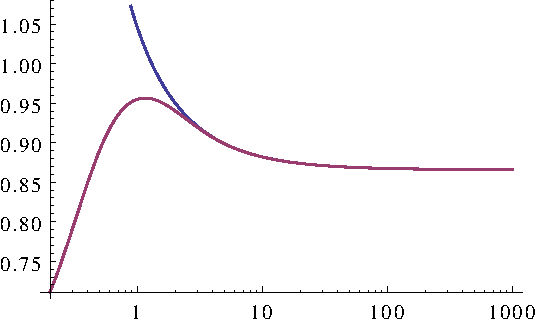
\includegraphics[width = 1 \textwidth]{plots/largelimit.pdf}
    \caption{Limit of $\alpha >>1$}
    \end{figure}
\end{minipage}\begin{minipage}[t]{0.49 \textwidth}
    \begin{figure}[H]
        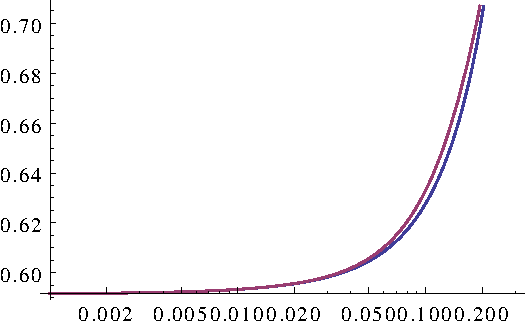
\includegraphics[width = 1 \textwidth]{plots/smalllimit.pdf}
    \caption{Limit of $\alpha <<1$}
    \end{figure}
\end{minipage}
\begin{figure}[H]
    \centering
    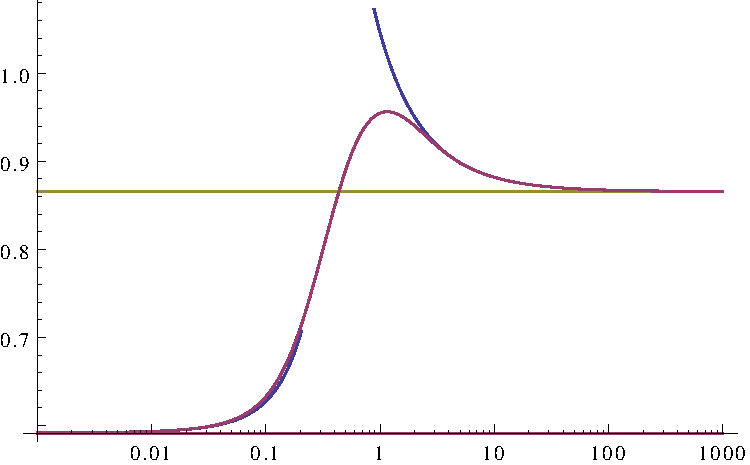
\includegraphics[width = 1 \textwidth]{plots/bothlimits.pdf}
    \caption{Limiting behaviour of Reaction Rate}
    \label{fig:rrlimit}
\end{figure}
It is obvious, that the reaction rate does not smoothly interpolate between the two limiting values but instead it has a local maximum. The obtained approximations for the limiting values can be used as a reasonable approximation.
\subsection{Effective Diffusivity Profile}
One approach to depict the effect of the barrier fluctuations to the particle movement is the calculation of an effective spatially depending diffusivity profile. Therefore the particles are assumed to move in a stable average potential such that they can be treated by means of the methods described in section \ref{The_Debye_Reaction_Rate}.\par
The total particle density is then given by
\begin{equation}
    \rho(r) = K\exp \left[ -\frac{U_m(r)}{K_B T} \right] \int_{R_s}^{r} \frac{\exp \left[ \frac{U_m(r')}{K_B T}\right]}{4 \pi D(r')r'^2} {\rm d} r'
\end{equation}
Where $K$ is now the actual absorption rate at the sink boundary, $U_m$ is the mean potential of the barrier and $D(r)$ is the spatially depending diffusion constant. To derive an expression for $D(r)$ we derivate by $r$ and invert the resulting equations:
\begin{align*}
    \rho'(r) &= -K\frac{U'_m(r)}{K_B T}\exp \left[ \frac{U_m(r)}{K_B T} \right] \int_{R_s}^{r} \frac{\exp \left[ \frac{U_m(r')}{K_B T}\right]}{4 \pi D(r')r'^2} {\rm d} r' + K \exp\left[ \frac{U_m(r)}{K_B T} \right] \frac{\exp \left[ \frac{U_m(r)}{K_B T}\right]}{4 \pi D(r')r^2} \\
\rho'(r) &= \frac{K}{4 \pi D(r) r^2} \\
\rho'(r) &= \frac{4 \pi D(R_s) R_s^2 \rho(R_s)}{4 \pi D(r) r^2}
\end{align*}
Such that for the diffusivity profile is given by
\begin{equation}
    \frac{D(r)}{D(R_s)} = \frac{4 \pi R_s^2 \rho'(R_s)}{ 4 \pi r^2 \rho'(r)}.
    \label{spatial_diffusivity_profile}
\end{equation}


\subsection{Resonant activation}
From the signs of the coefficients of the first order correction to the limits of the reaction rate for $\alpha>>1$ and $\alpha<<1$ it becomes obvious that this resonant behaviour always appears. Since the slope of the reaction rate is positive in both limits there must be a certain value of $\alpha$ that maximises the reaction rate. This effect has been observed in escape and first passage time problems and is known as \textit{Resonant Activation}.
In the next sections we will take a closer look to some limiting cases. Hopefully, this will lead to a better understanding of the behaviour of the system and point out features that are essential for the resonance to appear.

\subsection{The ideal two state Barrier}

The first limit we take is the one of an ideal barrier. Therefore we take $|u| \rightarrow \infty$ and obtain for the Rate
\begin{equation}
    \frac{1}{K_{Debye}}\lim_{u \rightarrow \infty}K = \frac{K^{+}}{K_{Debye}} = \frac{F_{1}^{+}}{F_{2}^{+}}
    \label{K+}
\end{equation}
\begin{align*}
    F_{1}^{+} = -(b \alpha+1)  & \left( 2 b \alpha e^{\alpha (a+b+2)}-2 b \alpha e^{\alpha (3 a+b)}+(a \alpha+1) e^{2 (b+1) \alpha} \right. \\
                                & \left.+(3 a \alpha-1) e^{2 \alpha (a+b)} -e^{2 (a+1) \alpha} (3 a \alpha+1)+e^{4 a \alpha} (1-a \alpha) \right)
\end{align*}
\begin{align*}
    F_{2}^{+} = & 2 \alpha e^{\alpha (a+b+2)} \left(a^2 \alpha-a \alpha+a-b \alpha-2\right)+2 \alpha e^{\alpha (3 a+b)} \left(a^2 \alpha-a (\alpha+1)+b \alpha+2\right) \\
                &-e^{2 \alpha (a+b)} \left(3 \alpha^2 (a (b-2)+2 b)+\alpha (a-3 b+4)-1\right)+e^{4 a \alpha} (a \alpha-1) (b \alpha+1) \\
                &+e^{2 (a+1) \alpha} ((a+2) \alpha+1) (b \alpha+1)-(a \alpha+1) e^{2 (b+1) \alpha} ((3 b-2) \alpha+1)
\end{align*}
In the positive limit and 
\begin{equation}
    \frac{1}{K_{Debye}} \lim_{u \rightarrow -\infty}K = \frac{K^{-}}{K_{Debye}} =  \frac{F_{1}^{-}}{F_{2}^{-}}
        \label{K-}
\end{equation}

\begin{align*}
    F_{1}^{-} + &-2 b \alpha (b \alpha+1) e^{\alpha (a+b+2)}+2 b \alpha (b \alpha+1) e^{\alpha (3 a+b)}+e^{4 a \alpha} (a \alpha-1) (b \alpha+1)- \\
                &e^{2 (a+1) \alpha} (a \alpha-1) (b \alpha+1)+(a \alpha+1) e^{2 (b+1) \alpha} (3 b \alpha-1)-(a \alpha+1) (3 b \alpha-1) e^{2 \alpha (a+b)}
\end{align*}
\begin{align*}
    F_{2}^{-} = & 2 \alpha e^{\alpha (a+b+2)} \left(a^2 \alpha-a \alpha+a-b \alpha-2\right)+2 \alpha e^{\alpha (3 a+b)} \left(a^2 \alpha-a (\alpha+1)+b \alpha+2\right) \\
                &-e^{2 \alpha (a+b)} \left(\alpha^2 (a (3 b+2)-2 b)+\alpha (-3 a+b+4)-1\right)+e^{4 a \alpha} (a \alpha-1) (b \alpha+1) \\
                &-e^{2 (a+1) \alpha} ((3 a-2) \alpha-1) (b \alpha+1)+(a \alpha+1) e^{2 (b+1) \alpha} ((b+2) \alpha-1)
\end{align*}
In the negative limit. The following plots demonstrate the behaviour of the system in the limiting cases.
\newpage
\begin{minipage}[t]{0.7 \textwidth}
    \begin{figure}[H]
        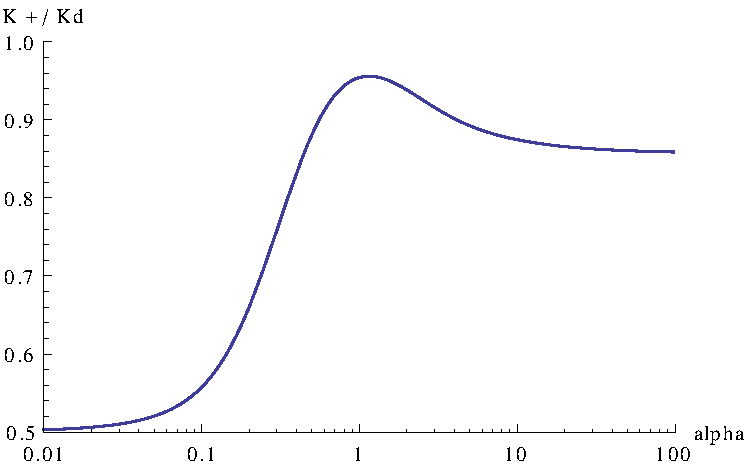
\includegraphics[width = 1 \textwidth]{plots/K+.pdf}
    \caption{Normalized reaction rate vs. switching rate for \newline repulsive barrier in the limit of $u \rightarrow \infty$,\newline parameters: $a = 4$, $b = 6$}
    \end{figure}
\end{minipage}\begin{minipage}[t]{0.3 \textwidth}
    The plot on the left shows the reaction rate relative to the reaction rate of the ungated Debye problem for a fluctuating potential barrier of hight $[U_1 = 0, U_2 = \infty]$. It is obvious that it does not show any qualitative differences from the system with a fluctuating barrier of finite hight as illustrated in figure \ref{fig:finite_barrier_rate+}. The reaction rate does still converge to finite constant values for infinitely slow or fast potential switching rates and takes a maximum value in between.
\end{minipage}

\begin{minipage}[t]{0.7 \textwidth}
    \begin{figure}[H]
        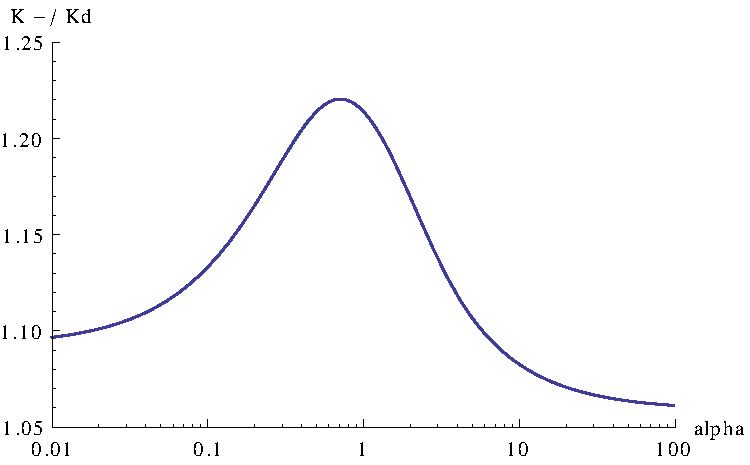
\includegraphics[width = 1 \textwidth]{plots/K-.pdf}
    \caption{Normalized reaction rate vs. switching rate for \newline attractive barrier in the limit of $u \rightarrow - \infty$,\newline parameters: $a = 4$, $b = 6$}
    \end{figure}
\end{minipage}\begin{minipage}[t]{0.3 \textwidth}
    This plot shows the quotient of the reaction rates of the gated and the ungated Debye problem for an attractive fluctuating potential barrier of hight $[U_1 = 0, U_2 = -\infty]$. As in the previous case the qualitative behaviour of the system does not change compared to the case of a finitely high potential (comp. figure \ref{fig:finite_barrier_rate-}). 
\end{minipage}

\begin{itemize}
    \item Therefore we conclude that \textit{the finite hight of the potential barrier is not essential for the appearance of resonant activation in reaction rates}.
\end{itemize}
Now that we have seen that the magnitude of the potential barrier does not alter the system qualitatively (as long as it does not equal zero) we will test other possible feature of the system on their significance regarding resonant activation. 

\subsection{The one dimensional Limit}

The question is now: does the local curvature of the potential barrier matter or does the system still show resonant activation if it is approximated by an absorbing wall and a flat fluctuating barrier.
Before we use advanced methods such as path integrals to investigate the simplified problem we will find out, if there is something to find out at all.
Therefore we continue from the limits on an ideal barrier \eqref{K+} and \eqref{K-} and substitute
\begin{equation}
    a \Rightarrow 1+t, \qquad b = a + gt.
    \label{Substitution}
\end{equation}
\par
The gap between sink and barrier $t$ is given in units of the sink radius $R_s$. The barrier itself is $gt$ wide. Now by taking $t/R_s \ll 1$ the radius of the system becomes very much larger than the length scale of the barrier width and distance from the sink. The radius of the sink therefore becomes equal to the curvature radius of the entire system. This way locally the situation is that of a fluctuating flat barrier in front of an absorbing wall. Lets see, if the resonant activation effect still persists.
\par
First consider the \textit{perfect repulsive barrier} as in \eqref{K+}. Substitution and Taylor expansion in $t$ to first order leads to
\begin{equation}
    \frac{\bar{K}^{+}}{K_{Debye}} = \frac{\alpha+1}{\alpha+2}-\frac{g t \alpha^2}{(\alpha+2)^2} 
    \label{K+linear}
\end{equation}
Obviously the first term is monotonously increasing and interpolates from 0.5 to 1. Now including the linear term in $t$ the expression does have a maximum at
\begin{equation}
    \alpha_m = \frac{2}{4t(g+1) - 1}.
    \label{alpham+}
\end{equation}
But a closer look reveals, that this maximum is positive only for $4t(g+1) < 1$ so only if $gt \approx 1$ which violates the assumptions we made in the first place when we did the Taylor expansion of equation \eqref{K+} for the reaction rate. 
\par
Now we consider the \textit{perfect attractive barrier} as in \eqref{K-}. We again substitute as in \eqref{Substitution} and do a Taylor expansion to first order in $t$ do derive
\begin{equation}
    \frac{\bar{K}^{+}}{K_{Debye}} = 1+\frac{g t}{4}.
    \label{K-linear}
\end{equation}
In this case the expression is fully independent from $/alpha$ and does solely depend on the geometric properties of the barrier-sink system.
\par
\begin{itemize}
    \item We conclude that the resonant activation effect can not be reproduced in a locally one dimensional approximation of the system. Therefore \textit{the spherical shape of the system must be critical for the emergence of resonant activation in reaction rates over metastable barriers}.
\end{itemize}
\subsection{Approximate Expressions for Resonant Potential Switching Rate}
As it is obvious from equation \eqref{two_state_rate} and following the search for an expression for the resonant transition rate of the potential barrier leads to transcendental equations that do not have an analytic solution. \\
Therefore we will try to find some approximative description for the resonant transition rate and compare it to numeric solutions of the equations that emerge from the derivative of the reaction rate in the limits of $|u| \rightarrow \infty$ as given in equation \eqref{K+} and \eqref{K-}.
\par
Until now we have identified two essential parameters in the system. First the \textit{decay length} in eq. \eqref{decay_length} and second the length scale of the barrier. Both are given in units of the sink radius. So it is only reasonable to assume that the condition for resonant activation to take place can be expressed in terms of these to system parameters. 
\par
In the following the transcendental equation
\begin{equation}
    \frac{\partial}{\partial \alpha} \frac{K^{+}}{K_{Debye}} = G^{+}(\alpha, t, g) = 0
    \label{dk+=0}
\end{equation}
has been subject to numerical evaluation for different $t$ and $g$ (comp. \eqref{Substitution}). The result is given in the following plot.
\begin{figure}[H]
    \centering
    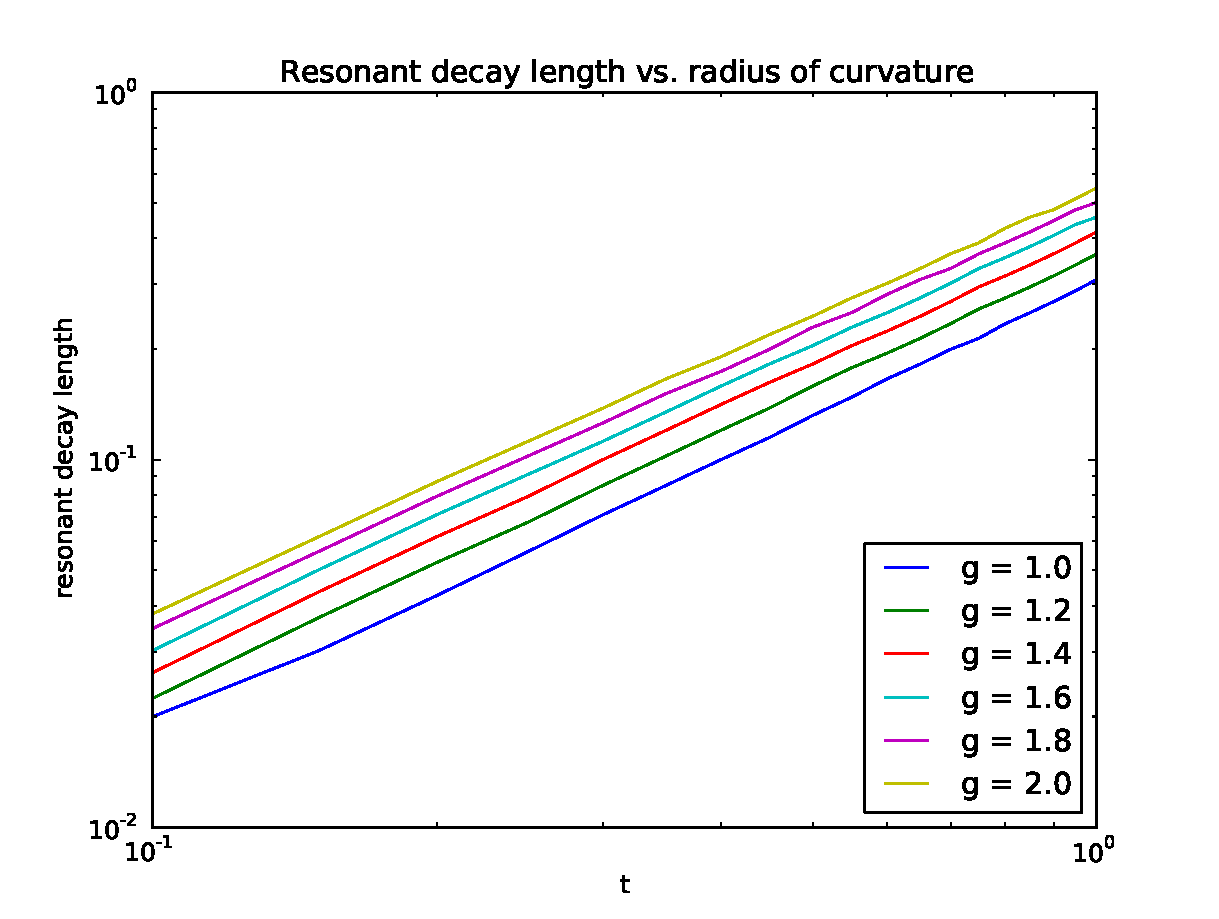
\includegraphics[width = 0.95 \textwidth]{plots/maxdclvst.pdf}
    \caption{Decay length $r_d$ vs system size $t$ at maximum absorption rate}
    \label{fig:maxdclvst}
\end{figure}
Both axis are have a logarithmic scale which makes it easily visible that there must be a power law of the form
\begin{equation}
    r_d^{(res)} = C \cdot t^{\kappa}
    \label{powerlaw}
\end{equation}
with $C$ and $\kappa$ being functions of $g$. Now the remaining task is to find expressions for the prefactor and exponent of the above \textit{empiric} relation.
The following plot displays the results of linear fits to the data presented in figure \ref{fig:maxdclvst}.
\begin{figure}[H]
    \centering
    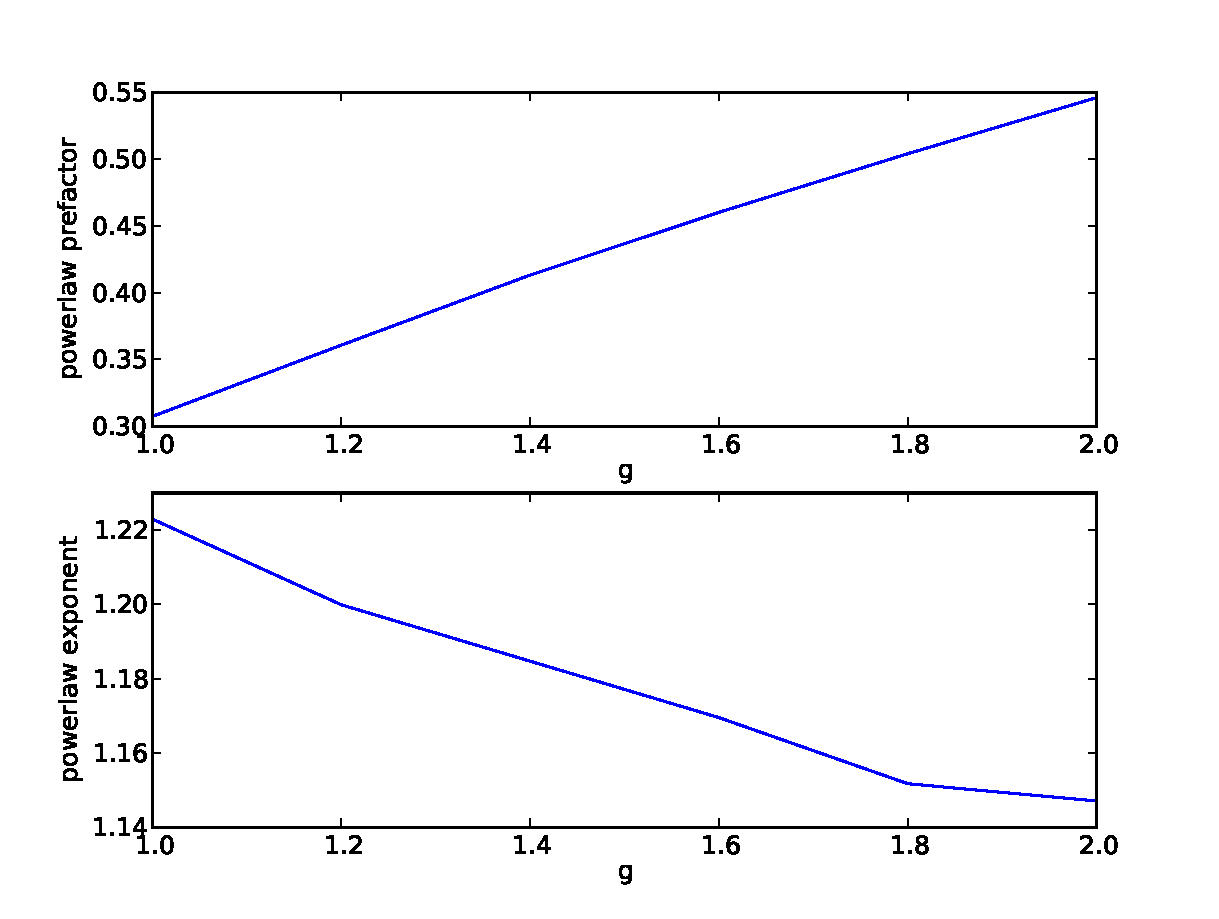
\includegraphics[width = 0.8 \textwidth]{plots/powerlawparameters.pdf}
    \caption{Values for $C$ and $\kappa$ obtained from fitting eq. \eqref{powerlaw} to data in fig \ref{fig:maxdclvst}}
    \label{fig:powerlawparameters}
\end{figure}
Now the preceding plots give rise to the assumption, that in the region of $t,g \approx 1$ a linear expansion in $g$ will give good results for $C$ and $\kappa$.\par
Numeric fits result in the linear equations for $C$ and $\kappa$:
\begin{align}
C(g) &= 0.313 + 0.239\cdot g \\
\kappa(g) &= 1.218 - 0.077 \cdot g
\end{align}
\begin{itemize}
    \item for $g,t \approx 1$ there is a power law connecting the \textit{decay length} to the length scale of the barrier,
    \item prefactor and exponent of the power law can be obtained from numeric evaluation of transcendental equations.
\end{itemize}

